\chapter{Vim} \label{ChapVim}
\pagenumbering{arabic}
\setcounter{page}{1}

%===============================================================
\section{Vim Tips and Tricks}
%===============================================================
Some good references are \cite{chang2018vim,toomey2015mastering}. A more
advanced tutorial that I haven't watched yet is \cite{chang2020vim}. A document
on effective text editing written by the creator of Vim can be found at
\cite{moolenaar2000seven}.
\begin{enumerate}
    \item In Linux based systems, put `setxkbmap -option "caps:escape' into
        ~/.bashrc to map the caps lock key to escape.
    \item To set Vim as your default text editor, use `sudo update-alternatives
        --config editor'.  \item Suppose the cursor is in the middle of a word.
        Whilst `cw' and `dw' will change/delete until the end of the word, `ciw'
        and 'diw' to change or delete the whole word, thereby not requiring you
        to move the cursor to the beginning of the word first.
    \item To reformat a paragraph, use `gq'. Reformatting includes enforcing the
        wrap limit which can be set in your vimrc with `set tw=\tlangle
        number\trangle'. Other options can be se such as indentation. Note that
        this command requires a minimum of two lines, so you'll need to at least
        use `gqj' and at most use `gjG' for the rest of the document under the
        line currently under the cursor.
    \item Use `m\tlangle key\trangle to set a mark to \tlangle key\trangle then
        \tlangle key\trangle to jump to it.  Note that if you set it to the
        capitalized version of \tlangle key\trangle then the jumping can occur
        between buffers. To see your list of marks, use `:mark'.
    \item Use `"\tlangle key\trangle' then an action like `y' or `d' to store
        text in the \textit{register} \tlangle key\trangle. Then use `"\tlangle
        key\trangle p' to paste it. Note that using `d' will automatically store
        it in the register at register x and `p' will automatically paste
        whatever is in register `x'.  Use `:reg' to see the register list.
    \item Use `f\tlangle key\trangle' to forward search for \tlangle
        key\trangle. To backwards search, use `F\tlangle key\trangle'. To repeat
        the search, use `;'.
    \item The `t' stands for `til'. For example, `dt=' will delete up to and not
        including an = sign.  \item The `*' can be used to search for the word
        under cursor.
    \item `J' is used to join the line below to the line currently under the
        cursor. This is useful for reformatting improperly wrapped lines but in
        general `gq' is more useful for this purpose.
    \item `zt' or `z\tlangle CR\trangle' will put the line under the cursor to
        the to of the window. `z.' will put the line to the center of the window
        and `z-' will put it to the bottom of the window.
    \item `z=' will give spelling suggestions for the word under the cursor.
    \item `[s' and `]s' to cycle backwards and forwards through misspelled words.
    \item Use `g\$' to go to the end of an unwrapped line.
    \item If you type a long line of text in insert mode, this counts as one
        action. Therefore, if you press undo, the whole line will be deleted. To
        break the undo chain, use \tlangle c-g\trangle u while in insert mode.
        Alternatively, you could map space to \tlangle c-g\trangle u so that the
        undo chain is broken whenever a space is added in insert mode:\\
        inoremap \tlangle Space\trangle \tlangle Space\trangle \tlangle
        c-g\trangle u
    \item Use the accent `\tlangle shift+6\trangle' in insert mode to move to
        the first non-white space character in the line.
    \item Use `\%' while your cursor is over a parenthesis, square or curly
        bracket to move to the corresponding open/closing parenthesis or
        bracket.
    \item Use `:ls' to see the list of buffers then `:b' and the number to
        select one. A useful mapping for this process is:\\ nnoremap \tlangle
        leader\trangle b:ls\tlangle cr\trangle:b\tlangle space\trangle
    \item Use `\tlangle number\trangle +\tlangle c-6\trangle' to switch to numbered buffer.
    \item Use `\tlangle c-f\trangle' in command line mode to view the command history in a
        buffer.
    \item In general, all yank, change or delete actions such as `y, c, d, x'
        etc will register the text object into the "" register. However, any
        yank action will also register the text object into the "0 register and
        any delete or change action will register the text object into the "-
        register.
    \item Use `s' or `S' to substitute. This is useful when you want to replace
        one letter with multiple letters.
    \item When using search `/\tlangle word\trangle', you can use \tlangle c-g
        \trangle and \tlangle c-t\trangle to cycle through them without
        confirming your search with \tlangle CR\trangle.
    \item Use `\tlangle c-r\trangle' in command line mode to paste from the
        register.
    \item Use `\tlangle c-r\trangle' in insert mode to paste from the register.
    \item Use \tlangle c-w\trangle N in a Vim terminal to switch to normal mode, which allows
        you to navigate as if you were in Vim.
    \item Use `\tlangle c-z\trangle' to suspend Vim and return to shell. Use `fg'
        in shell to resume the suspended program. You can also use
        \begin{lstlisting}
            stty susp undef
            bind '"\C-z":"fg\015"'
        \end{lstlisting}
        in your bashrc to, overall, set `\tlangle c-z\trangle' to toggle a
        suspended progran.
    \item Using `ctags -R' in terminal creates a tag file. Then, in vim, use
        `\tlangle c-$]$ \trangle' while the cursor is over a function name to
        jump to the code defining the function. You can also add the following
        shortcut to your vimrc:
        \begin{lstlisting}
            command! MakeTags !ctags -R .
        \end{lstlisting}
        so that tags can be created from the command line within Vim.
        Note that you need to add
        \begin{lstlisting}
            set tags=tags;/
        \end{lstlisting}
        to your vimrc so that ctags will check the current folder for tags file
        and keep going one directory all the way to root folder. See
        \cite{ben2011ctags} for more details.
\end{enumerate}

%===============================================================
\section{Plugin Management}
%===============================================================
The first part of this section follows \cite{neil2010synchronizing}. First, we
work towards turning ~/.vim into a git repository:
\begin{enumerate}
    \item Move \tsim/.vimrc into \tsim/vim.
    \item When vim boots, it's still going to look for .vimrc in the home
        directory. To ensure that it looks for vimrc in the \tsim/.vim
        directory, we can create a symbolic link to that file using `ln -s
        \tsim/.vim/vimrc \tsim/.vimrc'.  \item Make \tsim/.vim into a git
        repository.
\end{enumerate}
An issue now is if you install a plugin that itself is a git repository, you
lose the version-control capabilities of that plugin. To circumvent this issue,
we use a plugin manager; in this case \textit{Pathogen}.\\

%---------------------------------------------------------------
\subsection{Pathogen} \label{SecPathogen}
%---------------------------------------------------------------
The pathogen plugin makes it possible to cleanly install plugins as a bundle.
Rather than having to place all of your plugins side by side in the same
directory, you can keep all of the files for each individual plugin together in
one directory (see video from first link for example). This makes installation
more straightforward, and also simplifies the tasks of upgrading and even
removing a plugin if you decide you no longer need it since they are carefully
segregated from each other. For a good tutorial on Pathogen, see
\cite{lafourcade2014how}.\\

Following the readme on the repo at \cite{pope2009pathogen}, to install Pathogen
do the following:
\begin{enumerate}
    \item Run in terminal:\\
        mkdir -p \tsim/.vim/autoload \tsim/.vim/bundle \&\& \ \\ curl -LSso
        \tsim/.vim/autoload/pathogen.vim https://tpo.pe/pathogen.vim
    \item Add the following to your vimrc:
        execute pathogen\#infect()
\end{enumerate}
Now any plugins you wish to install can be extracted to a subdirectory under
~/.vim/bundle, and they will be added to the 'runtimepath'. For example, to
install "sensible.vim", simply run: "cd ~/.vim/bundle \&\& \ git clone
https://github.com/tpope/vim-sensible.git".

%---------------------------------------------------------------
\subsection{Submodules: Installing Git Repositories Within Git Repositories}\label{SecSubmodules}
%---------------------------------------------------------------
This section follows \cite{neil2010synchronizing}. Now that we can install
plugins via Pathogen, let's see how we preserve the version control capabilities
of our plugins. As a worked example, let us install the \textit{Vimtex} plugin:
\begin{enumerate}
    \item cd \tsim/.vim
    \item Now to clone a git repository into the bundle directory, use:\\ git
        submodule add https://github.com/lervag/vimtex.git bundle/vimtex
\end{enumerate}
Now, to upgrade this plugin, use:
\begin{enumerate}
    \item cd \tsim/.vim/bundle/vimtex
    \item git pull origin master
\end{enumerate}
To update ALL of your plugins, use:
\begin{enumerate}
    \item cd \tsim/.vim
    \item git submodule foreach git pull origin master
\end{enumerate}
%---------------------------------------------------------------
\subsection{Importing Your Vim Configuration and Plugins To a New Machines}
%---------------------------------------------------------------
One of the main benefits of version controlling your Vim configuration and
plugins is the ease of which they can be imported into a new machine. To do so,
use the following:
\begin{enumerate}
    \item cd \tsim
    \item git clone \tlangle git repo url\trangle \tsim/.vim
    \item ln -s \tsim/.vim/vimrc \tsim/.vimrc
    \item cd \tsim/.vim
    \item git submodule init
    \item git submodule update
\end{enumerate}
%---------------------------------------------------------------
\subsection{Vim-plug}
%---------------------------------------------------------------
Whilst Pathogen is the most basic plugin manager, there are limitations when
porting your setup to a new machine:
\begin{enumerate}
    \item When you run git submodule update, you'll pull the latest versions of
        the plugins from their respective repositories. So unless you've noted
        down somewhere all the commit IDs for your favourite version of each
        plugin, your overall plugin collection cannot be preserved when porting
        to a new machine.
    \item Suppose one of the plugins is no longer being maintained by the owner
        and suppose also that you've made your own changes to the plugin. If you
        were to pull your configuration on a new machine, you will pull the
        latest version of the plugin; that is your changes will not be ported.
        Further, on your own repository for your configuration, the directories
        containing the plugins will be treated as repositories. Unless you
        manually install the plugins, there is no way to preserve your changes
        onto Github.
\end{enumerate}
The plugin manager Vim-plug \cite{junegunn2014vimplug} has a solution to the
first problem. This plugin manager is extremely simple to use:
\begin{enumerate}
    \item Run in terminal:\\
        curl -fLo \tsim/.vim/autoload/plug.vim --create-dirs \
        https://raw.githubusercontent.com/junegunn/vim-plug/master/plug.vim
    \item In your vimrc, add the line:\\
        call plug\#begin('\tsim/.vim/plugged')
    \item To include a plugin you wish to install under the line above, in your
        vimrc add the following line:\\
        Plug 'https://github.com/lervag/vimtex.git'
    \item Under `Plug \tlangle url \trangle' of your last plugin, in your vimrc
        add the following line:\\
        call plug\#end()
    \item Reload your vimrc and use the command `:PlugInstall' while in vim. Now
        all your plugins are installed.
\end{enumerate}
Now to preserve the versions of your plugin:
\begin{enumerate}
    \item In Vim, run the command `:PlugSnapshot! \tlangle filename \trangle.vim'.
    \item To restore the state of your plugins, in vim run the command:\\
        :source \tsim/.vim/\tlangle filename \trangle.vim\\
        or, in terminal:\\
        vim -S \tsim/.vim/\tlangle filename \trangle.vim
\end{enumerate}
See the bradagy's answer in the reddit post \cite{bradagy2018remember}. To port
your configuration to a new machine:
\begin{enumerate}
    \item cd \tsim
    \item git clone \tlangle git repo url \trangle \tsim/.vim
    \item cd \tsim/.vim/vimrc
    \item :PlugInstall
    \item :source \tsim/.vim/\tlangle filename \trangle.vim
\end{enumerate}
To uninstall plugins:
\begin{enumerate}
    \item Delete `Plug \tlangle url \trangle' line from your vimrc
    \item :PlugClean
\end{enumerate}
%===============================================================
\section{Native Plugin Management} \label{SecNativePluginManagement}
%===============================================================
Vim-plug provides a solution to the first of the two issues mentioned in the
previous section, but not the second. To address the second issue, we can use
Vim's native plugin management system to install a plugin and delete the .git
repository. That way, we can track the files and any changes in our own git
repository. This section follows \cite{shapeshed2019vim}. For a more
detailed explanation, see \cite{manasthakur2020managing} or \cite{ryder2018attack}.\\

The package feature of Vim 8 follows a pathogen-like model and adds the plugins
found inside a custom-path \tsim/.vim/pack/ to Vim's runtime path. You can check
the version of Vim installed using `vim --version'. To install using this native
feature, we use the following steps:
\begin{enumerate}
    \item mkdir -p \tsim/.vim/pack/plugins/start/
    \item cd \tsim/.vim/pack/plugins/start/
    \item git clone \tlangle url\trangle or git submodule add \tlangle url
        \trangle
\end{enumerate}
and that's it! To remove a plugin, simply remove its directory: rm -r
\tsim/.vim/pack/plugins/start/\tlangle plugin\_directory\_name \trangle if the
plugin was cloned. Or, if it was added as a submodule, use:
\begin{enumerate}
    \item git submodule deinit vim/pack/shapeshed/start/\tlangle plugin\_directory\_name \trangle
    \item git rm vim/pack/shapeshed/start/\tlangle plugin\_directory\_name \trangle
    \item rm -Rf .git/modules/vim/pack/shapeshed/start/\tlangle plugin\_directory\_name \trangle
\end{enumerate}
To import your vim configuation and plugins to your new machine, simply use the
same steps as required for Pathogen:
\begin{enumerate}
    \item cd \tsim
    \item git clone \tlangle git repo url\trangle \tsim/.vim
    \item ln -s \tsim/.vim/vimrc \tsim/.vimrc
    \item cd \tsim/.vim
    \item git submodule init
    \item git submodule update
\end{enumerate}
and also, to update all your plugins, you again use
\begin{enumerate}
    \item cd \tsim/.vim
    \item git submodule foreach git pull origin master
\end{enumerate}
If you have your own plugins that are not cloned from external repositories
(i.e. you've written your own .vim files), you can simply create a directory
~/.vim/plugin and copy your plugins into there.\\

In conclusion, although Pathogen seems to be the most cumbersome, it could be
the case that the servers do not have Vim 8 installed and so the native plugin
manager will not work nor do they allow Vim-plug to install plugins. In such a
case, Pathogen is your best bet.

%===============================================================
\section{Vimtex}
%===============================================================
This section discusses the Vimtex \cite{lervag2015vim} plugin. See also the
vimways article \cite{woodruff2019latex} for a good overview.  To install MikTex
into Linux, run ``sudo apt-get install texlive-full''.

%---------------------------------------------------------------
\subsection{Installing and Running Vimtex}
%---------------------------------------------------------------
Assuming you are using the Pathogen plugin manager and version controlling your
~/.vim directory, follow the steps used in Section \ref{SecSubmodules}. Then use
`:Helptags' which is Pathogen's method for generating help tags. With this, we
can use `:h vimtex' to see the manual for Vimtex. To confirm that the plugin
works, type ":VimtexInfo" to see a summary of the tex file.
%---------------------------------------------------------------
\subsection{Compiling a Tex File}
%---------------------------------------------------------------
The following commands are useful:
\begin{itemize}
    \item :VimtexCompile \# this is a continuous compiler meaning that everytime
        you save with ":w" it will automatically compile
    \item :VimtexStop \# this stops the continuous compiler
    \item :VimtexCompileSS \# this is a single shot compiler. Note that you have
        to save your file first \item :VimtexClean \# Cleans auxiliary files
        generated in compilation process
\end{itemize}
I set the following mappings in my vimrc:
\begin{lstlisting}
autocmd FileType tex nnoremap <F5> :VimtexView<CR>
autocmd FileType tex inoremap <F5> <Esc> :VimtexView<CR>
autocmd FileType tex nnoremap <F6> :w! <bar> :VimtexCompileSS<CR>
autocmd FileType tex inoremap <F6> <Esc> :w! <bar> :VimtexCompileSS<CR>
\end{lstlisting}
Here are some useful commands I use in my vimrc:
\begin{lstlisting}
" Avoids opening an empty .tx file only to have vimtex recognize it as plain Tex rather than Latex
    let g:tex_flavor = 'latex'

" Use folding. Use zx to unfold and zX to fold all
    let g:vimtex_fold_enabled = 1

" Toggle Error Window On and Off
    autocmd FileType tex map <F4> \le

" Shortcut for Compiling and Viewing PDF
    autocmd FileType tex nnoremap <F5> :VimtexView<CR>
    autocmd FileType tex inoremap <F5> <Esc> :VimtexView<CR>
    autocmd FileType tex nnoremap <F6> :w! <bar> :VimtexCompileSS<CR>
    autocmd FileType tex inoremap <F6> <Esc> :w! <bar> :VimtexCompileSS<CR>

" VimtexClean on exit
  augroup vimtex_config
    au!
    au User VimtexEventQuit call vimtex#compiler#clean(0)
  augroup END
\end{lstlisting}
And here are some useful mappings for creating common math related LaTeX tex
objects:
\begin{lstlisting}
" Teleportation!
    autocmd FileType tex inoremap <Space><Space> <Esc>/<++><CR>"_c4l

" Inline Stuff
    autocmd FileType tex inoremap ;mm $$<++><Esc>5ha
    autocmd FileType tex inoremap ;bf \textbf{}<++><Esc>6hf}i
    autocmd FileType tex inoremap ;it \textit{}<++><Esc>6hf}i
    autocmd FileType tex inoremap ;bfs \boldsymbol{}<++><Esc>6hf}i
    autocmd FileType tex inoremap ;ct \cite{}<++><Esc>6hf}i
    autocmd FileType tex inoremap ;lb \label{}<++><Esc>6hf}i
    autocmd FileType tex inoremap ;rf \ref{}<++><Esc>6hf}i
    autocmd FileType tex inoremap ;erf (\ref{})<++><Esc>7hf}i

" Environments
    autocmd FileType tex inoremap ;itm \begin{itemize}<CR><CR>\end{itemize}<CR><++><Esc>2kA\item<Space>
    autocmd FileType tex inoremap ;enu \begin{enumerate}<CR><CR>\end{enumerate}<CR><++><Esc>2kA\item<Space>
    autocmd FileType tex inoremap ;aln \begin{align}<CR><CR>\end{align}<CR><++><Esc>2kA

" Math Environments
    autocmd Filetype tex inoremap ;def \begin{definition}<CR><CR>\end{definition}<CR><++><Esc>2kA
    autocmd Filetype tex inoremap ;thm \begin{theorem}<CR><CR>\end{theorem}<CR><++><Esc>2kA
    autocmd Filetype tex inoremap ;lem \begin{lemma}<CR><CR>\end{lemma}<CR><++><Esc>2kA
    autocmd Filetype tex inoremap ;cor \begin{corollary}<CR><CR>\end{corollary}<CR><++><Esc>2kA
    autocmd Filetype tex inoremap ;prp \begin{proposition}<CR><CR>\end{proposition}<CR><++><Esc>2kA
    autocmd Filetype tex inoremap ;prf \begin{proof}<CR><CR>\end{proof}<Esc>1kA

" Math Stuff
    autocmd Filetype tex inoremap ;T ^\mathrm{T}
    autocmd FileType tex inoremap ;sd _{}<++><Esc>6hf}i
    autocmd FileType tex inoremap ;su ^{}<++><Esc>6hf}i
    autocmd FileType tex inoremap ;frc \frac{}{<++>}<++><Esc>12hf}i
    autocmd FileType tex inoremap ;mbb \mathbb{}<++><Esc>6hf}i
    autocmd FileType tex inoremap ;lrp \left(\right)<++><Esc>12hf(a
    autocmd FileType tex inoremap ;lrs \left[\right]<++><Esc>12hf[a
    autocmd FileType tex inoremap ;lrn \left\lVert\right\rVert<++><Esc>15hi<Space>
\end{lstlisting}

%---------------------------------------------------------------
\subsection{Forward and Backwards Searching with Synctex}
\label{SecFwdBckwdSynctex}
%---------------------------------------------------------------
This section follows \cite{gunther2014vimtex}. For this, you will need a Vimtex
server which allows you to do forward and backward to navigate between
corresponding sections of the tex file and the pdf. You will also need the pdf
viewer \textit{Zathura}. To install, simply use `sudo apt-get install zathura'.
Then, in your vimrc, add the following line `let g:vimtex\_view\_method =
'zathura''.\\

Following \cite{lerner2004enable}, to install just use `sudo apt-get install
vim-gnome'. Finally, to edit a tex file with navigation capabilities:
\begin{enumerate}
    \item In the directory containing the tex file, use:\\
        vim --servername \tlangle servername\trangle \tlangle texfile\trangle.tex
    \item While in tex file, to jump to the text on the pdf corresponding to the
        line under your cursor, use:\\
        \tlangle leader\trangle lv
    \item Move your mouse cursor over some text on the pdf. Then, to jump to
        corresponding text on the tex file, use:\\
        Ctrl + left-click
\end{enumerate}
Note that \tlangle leader\trangle lv forward search works without the Vim
server; it's the backwards search that requires the Vim server.\\

Note that as of at least July 1st 2021, vim-gnome no longer exists.
Instead, use vim-gtk which can be installed with `sudo apt-get install
vim-gtk'.

%---------------------------------------------------------------
\subsection{Other Useful References}
%---------------------------------------------------------------
\begin{itemize}
    \item Good article overviewing Vimtex \cite{woodruff2019latex}
    \item Nice compilation of Vimtex commands \cite{gunther2014vimtex}
    \item Quick guide on the basics of Vimtex \cite{jdhao2019complete}
    \item For a comparison with other Vim LaTeX plugins \cite{lervag2015vim}
    \item Some useful mappings such as the teleportation trick
        \cite{smith2016my, smith2017start}.
    \item Note-taking using Vim and LaTeX for math lectures \cite{castel2019how}
    \item Vim and LaTeX on MacOS \cite{dyke2020getting}
\end{itemize}

%===============================================================
\section{IPython}
%===============================================================
The following mapping may prove useful for starting an IPython terminal in
Vim:\\
\begin{lstlisting}
nnoremap <leader>P :botright vertical terminal ipython --no-autoindent<CR><C-w><left>
\end{lstlisting}

%---------------------------------------------------------------
\subsection{sendtowindow Plugin}
%---------------------------------------------------------------
When coding in Python with a Vim terminal on the side running IPython, I use the
\textit{sendtowindow} plugin \cite{KKPMW2016send} to send lines of code to the
terminal. See \cite{KKPMW2019send} for a Reddit post from the author discussing
the plugin. It's a very simple plugin that allows the use of vim motions to move
lines of text to terminals left, right, above or below the Vim window. I use the
following maps:\\
\begin{lstlisting}
let g:sendtowindow_use_defaults=0
nmap ,sr <Plug> SendRight
xmap ,srv <Plug> SendRightV
nmap ,sl <Plug> SendLeft
xmap ,slv <Plug> SendLeftV
nmap ,su <Plug> SendUp
xmap ,suv <Plug> SendUpV
nmap ,sd <Plug> SendDown
xmap ,sdv <Plug> SendDownV
\end{lstlisting}
Note that these mappings must not be noremaps (mappings that are non-recursive). For an
explanation on why this is the case, please see \cite{justrajdeep2018please}.
Any one of these mappings will specify to either send some text in normal mode
or in visual mode. When in normal mode, to specify which text to send, use the
usual Vim movements. For example, `,sr\$' will send from the cursor to the end
of the line to the window on the right. However, if you are in the middle of a
line, it may become tedious having to first go to the beginning of the line and
having to type `\$'. Therefore, we can define line objects using the following
maps:
\begin{lstlisting}
onoremap <silent> <expr> - v:count==0 ? ":<c-u>normal! 0vg_<CR>" : ":<c-u>normal! V" . (v:count) . "jk<CR>"
onoremap <silent> <expr> i- v:count==0 ? ":<c-u>normal! ^vg_<CR>" : ":<c-u>normal! ^v" . (v:count) . "jkg_<CR>"
\end{lstlisting}
With '-' alone the indentation is left intact and 'i-' is without indentation.
So, for example, `,sr-' will send the line under the cursor to the window on
the right with indentation and `,sr8-' will send four lines under the cursor to
the window on the right with indentation. Note that this is important for Python as if you try
send a for loop with `i-' and leave out the indentation, then it may not run.\\

I have extended the plugin with SendTextToTerminalRight command and SendVariableRight()
and SendMarkedSectionRight() functions (I've also coded for the other three directions as
well). Using these, we can send clear, \%reset and run code commands as well as
variable and marked sections of code to the IPython terminal.
\begin{lstlisting}
" sendtowindow for IPython in Vim Terminal: clear, reset, run code, run variable, run marked section
    noremap ,sL :SendTextToTerminalRight clear<CR>
    noremap ,sD :SendTextToTerminalRight %reset -f<CR>
    noremap ,sR :w!<CR>:SendTextToTerminalRight run <c-r>%<CR>
    nmap ,sV <Plug>SendVariableRight
    nmap ,sM <Plug>SendMarkedSectionRight
\end{lstlisting}
For the map that runs the Python code, we leverage the fact that
`\tlangle c-r\trangle' in command mode will prime pasting from the register and
\% in the register stores the file name.\\

The SendMarkedSectionRight() function has been coded such that the section must
be marked with `x' on the top of the section and `z' on the bottom.  The plugin
vim-signature \cite{kshenoy2015signature} may come in handy for manipulating the
marks. In particular, the plugin displays marks and the command `dm\tlangle mark
name\trangle' deletes the mark; so `dmq' above deletes the mark called `q'.

%---------------------------------------------------------------
\subsection{Slimux plugin}
%---------------------------------------------------------------
There are many plugins that allow interaction between Vim and tmux. For example,
there is Vim-Slime \cite{jpalardy2012slime} and Vimux \cite{benmills2009vimux}.
The one I use is Slimux \cite{esamattis2015slimux}. There is a blog post about
it here \cite{suuronen2012slimux}. As discussed in the blog post, Slimux differs
from Vimux in that it is more disjoint from tmux. In particular, Vimux will
create a pane on which you must run your commands whereas Slimux allows you to
select the pane you wish to use. Also, unlike Vim-Slime, you do not need to
manually type in the pane to select it; in Slimux an interactive prompt is
given. It's also worth noting that Vim-Slime supports many terminal multiplexers
such as GNU Screen, kitty and Vim's native terminal.\\

However, with Slimux, there is an issue with sending commands to IPython where the
indentation is constantly carried over \cite{kmARC2015indentationerror}. There
are three proposed fixes
\cite{lotabout2017remove,karadaharu2016add,zcesur2018fix}. The first modifies
python.vim, the second modifies both slimux.vim and python.vim by implementing
IPython's cpaste function and the third modifies a single line of slimux.vim.
Since the repo owner hasn't pulled any of these fixes, I opted for the third fix
which requires changing line 328 of slimux.vim in the SlimuxSendCode() function:
\begin{lstlisting}
let b:code_packet["text"] = a:text
\end{lstlisting}
to:
\begin{lstlisting} let
b:code_packet["text"] = "\e[200~" . a:text . "\e[201~\r\r.
\end{lstlisting}
There is also an issue with the SlimuxSendKeys() function. This function sends
keys to the terminal using the `tmux send-keys' syntax. A simple fix is to
change line 228 of slimux.vim from
\begin{lstlisting}
call system(g:slimux_tmux_path . ' send-keys -t " . target . " " . keys)
\end{lstlisting}
to
\begin{lstlisting}
call system(g:slimux_tmux_path . " send-keys -t " . target . " " . keys)
\end{lstlisting}
It's surprising that this small typo went unnoticed. Note that this repository has not
been updated in years and so all pull requests have not been fulfilled.
Therefore, if you wish to track the fixes you've made, you may want to install
the plugin manually so that it does not follow the original repository. This was
disussed in Section \ref{SecNativePluginManagement}.\\

I use the following mappings:
\begin{lstlisting}
" Primer for Vim motions to select text to be sent
    nmap ,t <Plug>SlimuxREPLSendWithMotion

" Send text selected in visual mode
    vnoremap ,t :SlimuxREPLSendSelection<CR>

" Send terminal commands
    nnoremap ,tX :SlimuxShellPrompt<CR>
    nnoremap ,tT :SlimuxShellRun<Space>
    nnoremap ,tE :SlimuxShellRun exit<CR>

" Send keys using the 'tmux send-keys' syntax
    nnoremap ,tK :SlimuxSendKeys<Space>
    nnoremap ,tC :SlimuxSendKeys<Space>c-c<CR>

" Slimux for IPython in tmux terminal : IPython, clear, reset, run code, run variable, run marked section
    nnoremap ,tP :SlimuxShellRun ipython<CR>
    nnoremap ,tL :SlimuxShellRun clear<CR>
    nnoremap ,tD :SlimuxShellRun %reset -f<CR>
    nnoremap ,tR :w!<CR>:SlimuxShellRun run <c-r>%<CR>
    nmap ,tV <Plug>SlimuxREPLSendVariable
    nmap ,tM <Plug>SlimuxREPLSendMarkedSection
\end{lstlisting}
where SlimexShellRun awaits a command to send to shell and SLimuxSendKeys sends
key inputs using the 'tmux send-keys' syntax. The SlimuxREPLSendWithMotion was
not part of the original slimux plugin. My code is as follows:
\begin{lstlisting}
function! s:GetTextWithMotion(type)
  let s:saved_registert = @t

  " Obtain wanted text
  if a:type ==# "char"
    keepjumps normal! `[v`]"ty
    call setpos(".", getpos("']"))
  elseif a:type ==# "line"
    keepjumps normal! `[V`]$"ty
    call setpos(".", getpos("']"))
  endif
  let text = @t

  " Restore register
  let @t = s:saved_registert

  return text
endfunction

function! s:SlimuxREPLSendWithMotion(type)
   let text = s:GetTextWithMotion(a:type)
   call SlimuxSendCode(text)
endfunction

nnoremap <silent> <Plug>SlimuxREPLSendWithMotion :<C-U> set operatorfunc=<SID>SlimuxREPLSendWithMotion<CR>g@
\end{lstlisting}
The `g@' sets the mark `[' at the beginning of the motion and `]' at the end of
the motion. This can then be leveraged in functions. The `@' in the context of
functions refers to the register.

%---------------------------------------------------------------
\subsection{Other Useful References}
%---------------------------------------------------------------
\begin{itemize}
    \item A good Reddit thread on workflow with Vim and IPython can be found at
        \cite{abdeljalil732020anyone}. Note that the majority of the responses
        indicate that they use vim-slime and tmux.
    \item The vim-tmux-runner plugin \cite{toomey2013tmuxrunner} may be worth checking out.
    \item The vim-ipython-cell plugin \cite{hanschen2019ipython} may be worth
        checking out. There is a reddit post \cite{hanschen2019reddit} by the
        author on this plugin. Note that this plugin is leverages vim-slime.
        According to the author, the main contribution of this plugin is that it
        provides many ways to define and run cells, even using Vim marks.
    \item Another lightweight workflow can be found in
        \cite{hornung2019boosting}. For this, you will need three plugins: Vimux
        \cite{benmills2009vimux}, vim-pyShell \cite{hornung2019pyShell} and
        vim-cellmode \cite{julienr2016vimcellmode}. However, I have trouble
        getting this to work. Starting and stopping a pyShell session works fine
        as well as sending one line of code, but I have issues sending over
        cells.
\end{itemize}

%==============================================================================
\section{Autocompletion with YCM}
%==============================================================================
When deciding between \emph{You Complete Me (YCM)} \cite{ycmcore2017ycm} and
\emph{Conquer of Completion (CoC)} \cite{neoclide2020conquer}, I found the
following the discussion in \cite{desmap2020ycmvscoc} where a maintainer of YCM
details the design philosophy of YCM in the comments. Specifically, one of the
maintainers (puremourning) states that YCM prioritizes consistency, testing,
stability and performance over a range of functions such as snippet support of
insertion of parentheses. This appeals to me because honestly all I want is to
be able to jump to definition. Finally, as of writing this, I prefer to
out-source error checking to the compiler and linting to some external linting
program. Basically, I want my text-editor to just edit text and help me navigate
my code. With this in mind, YCM seems ideal as you can easily configure and
disable all these extra functions.\\

Another helpful resource was the video \cite{primeagen2020cocvsycm} where the
speaker uses both as YCM seems to perform better with TypeScript whilst CoC
performs better with C++. I'm not super sold on my choice, it was a bit of a
coin flip in the end, but I decided to go with YCM. Another possible option was
converting to Neovim and using it's native LSP, but I decided to hold out on the
conversion until Vim 9 is released.

%------------------------------------------------------------------------------
\subsection{Installation}
%------------------------------------------------------------------------------
I'm not entirely sure why the repository \cite{ycmcore2017ycm} suggests to use
Vundle accompanied by some complicated instructions. I instead found on
\cite{yves2020why} that you can simply include
\begin{lstlisting}
    Plug 'ycm-core/YouCompleteMe', { 'do': './install.py' }
\end{lstlisting}
into your vimrc. The installation process requires you to have `make' and
`cmake' which can be installed using the commands:
\begin{lstlisting}
sudo apt-get install build-essential
sudo apt install make
sudo apt-get -y install cmake
\end{lstlisting}
and also, even if you already have Python 3.8 installed, you may need:
\begin{lstlisting}
sudo apt-get install python-dev-is-python3
\end{lstlisting}
If you repeatedly see the error:
\begin{lstlisting}
YouCompleteMe ERROR: Python headers are missing in /usr/include/python3.9.
\end{lstlisting}
there may be an issue with Python. You can fix issues by running
\begin{lstlisting}
sudo apt install --reinstall python3 python python3-minimal --fix-broken
\end{lstlisting}

%------------------------------------------------------------------------------
\subsection{Mappings}
%------------------------------------------------------------------------------
Here are a few additions I made to the vimrc, beginning with the jump commands:
\begin{lstlisting}
    nnoremap <Leader>gd :YcmCompleter GoTo<CR>
    nnoremap <Leader>gr :YcmCompleter GoToReferences<CR>
    nnoremap <Leader>gi :YcmCompleter GoToImplementation<CR>
    nnoremap <Leader>gy :YcmCompleter GoToType<CR>
    nnoremap <Leader>rr :YcmCompleter RefactorRename<space>
\end{lstlisting}
The repository README provides a fantastic description of each of these
commands.\\

Additionally, I found configuring the behaviour to be a very elegant procedure:
\begin{lstlisting}
" Turn off automatic summoning of completion suggestions
    let g:ycm_auto_trigger = 0

" Completion Pop-Up Settings
    set pumheight=10
    set completeopt+=popup
    set previewpopup=height:10,width:60,highlight:PMenuSbar
    set completepopup=height:15,width:60,border:off,highlight:PMenuSbar
    let g:ycm_max_num_candidates_to_detail = 5
    let g:ycm_max_num_identifier_candidates = 5

" Disable preview at bottom of terminal when using completion
    set completeopt-=preview
    let g:ycm_add_preview_to_completeopt = 0

" If using preview, close window after using a selection
    let g:ycm_autoclose_preview_window_after_insertion = 1
    let g:ycm_autoclose_preview_window_after_completion = 1

" Disable summoning of documentation when hovering
    let g:ycm_auto_hover = ''

" Diagnostics UI settings
    let g:ycm_show_diagnostics_ui = 0
    let g:ycm_enable_diagnostic_signs = 0
    let g:ycm_enable_diagnostic_highlighting = 0
    let g:ycm_echo_current_diagnostic = 0
    let g:ycm_update_diagnostics_in_insert_mode = 0

" Commands to control completion pop up
    let g:ycm_key_invoke_completion = '<C-Space>'
    let g:ycm_key_list_stop_completion = ['<C-c>']

" Open Search
    nmap <Leader>F <plug>(YCMFindSymbolInWorkspace)

" Instead of triggering after hovering, summon documentation using a command
    nmap <Leader>D <plug>(YCMHover)

" Jumps
    nnoremap <Leader>G :YcmCompleter GoTo<CR>
    autocmd FileType python nnoremap <Leader>G :YcmCompleter GoToType<CR>
    nnoremap <Leader>gd :YcmCompleter GoToDefinition<CR>
    nnoremap <Leader>gy :YcmCompleter GoToType<CR>
    nnoremap <Leader>gi :YcmCompleter GoToImplementation<CR>
    nnoremap <Leader>gs :YcmCompleter GoToSymbol<CR>
    nnoremap <Leader>gr :YcmCompleter GoToReferences<CR>
    nnoremap <Leader>rr :YcmCompleter RefactorRename<space>
\end{lstlisting}
Some notes on this configuration. Firstly, for Python, both \textbf{GoTo} and
\textbf{GoToDefinition} just sends you to the import at the top of the file.
Intead, \textbf{GoToType} sends you to the file in which it was created.
Therefore, I instead specified a special map for when in Python files.\\

Interestingly enough, YCM does not offer the
ability to limit the number of suggestions displayed \cite{ioeric2019size}. To
be honest, I'm not entirely sure what the options:
\begin{lstlisting}
    let g:ycm_max_num_candidates_to_detail = 5
    let g:ycm_max_num_identifier_candidates = 5
\end{lstlisting}
do. Instead, you have to use a vanilla Vim configuration and decrease the size
of the window with
\begin{lstlisting}
    set pumheight=10
\end{lstlisting}
Now regarding the verbosity of the suggestions and the redundancy of its
appearance in the popup, there seems to be lengthy discourse over this in
\cite{dhleong2019abbreviate}. It doesn't seem like puremourning is in favour of
truncating the signatures following the idea that, without them, you can only
see details of the currently selected suggestion.

%------------------------------------------------------------------------------
\subsection{Python}
%------------------------------------------------------------------------------
You can find some detailed information about YCM with Python in the `Python
Semantic Completion' section of \cite{ycmcore2017ycm}. One idiosyncracy of
Python YCM must deal with is the use of virtual environments. There are two ways
offered by YCM:
\begin{itemize}
    \item A local solution. Create a \textbf{.ycm\_extra\_conf.py} file at the
        root directory of every project containing
        \begin{lstlisting}
            def Settings( **kwargs ):
            return {
                'interpreter_path': '/path/to/virtual/environment/python'
            }
        \end{lstlisting}
    \item A global solution. In your vimrc, add:
        \begin{lstlisting}
            let g:ycm_python_interpreter_path = ''
            let g:ycm_python_sys_path = []
            let g:ycm_extra_conf_vim_data = [
                \  'g:ycm_python_interpreter_path',
                \  'g:ycm_python_sys_path'
                \]
            let g:ycm_global_ycm_extra_conf = '~/global_extra_conf.py'
        \end{lstlisting}
        and create the \textbf{\tsim/global\_extra\_conf.py} file containing:
        \begin{lstlisting}
            def Settings( **kwargs ):
                client_data = kwargs[ 'client_data' ]
                return {
                    'interpreter_path': client_data[ 'g:ycm_python_interpreter_path' ],
                    'sys_path': client_data[ 'g:ycm_python_sys_path' ]
                }
        \end{lstlisting}
\end{itemize}
What this does is it sets all the paths you need for code jumps. Indeed, with
your file open in Vim, if you use \textbf{:YcmDebugInfo}, you'll be able to see
something like:
\begin{figure}[H]
    \centering
    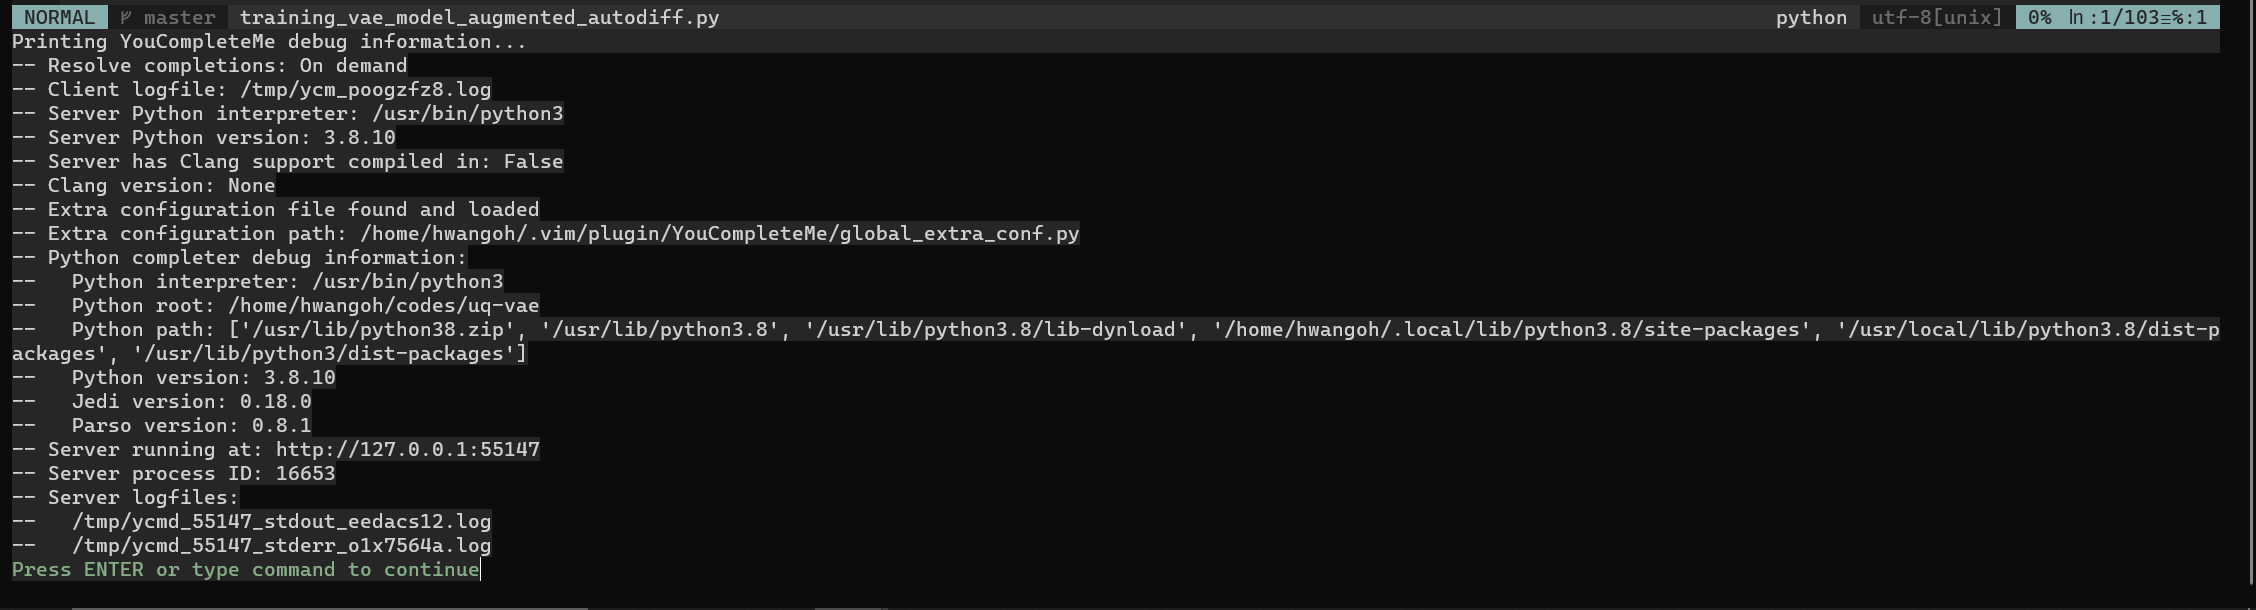
\includegraphics[scale=\figscale]{ycmdebuginfo.png}
    \caption{YCM debug information}
    \label{FigYcmDebugInfo}
\end{figure}
Notice in particular the `Extra configuration path' which I placed within
\textbf{\tsim/.vim/plugins/YouCompleteMe}.\\

One thing to take note of is that the code jumps may not work if you modify your
\textbf{sys.path} within the code. For example:
\begin{lstlisting}
import os
import sys
sys.path.insert(0, os.path.realpath('../../../src'))
sys.path.insert(0, os.path.realpath('..'))

# Import src code
from utils_io.filepaths_vae import FilePathsTraining

# Import Project Utilities
from utils_project.filepaths_project import FilePathsProject
\end{lstlisting}
Here, I have modified the path such that I can abbreviate the import of
\textbf{../../../src/utils\_io/filepaths\_vae} to simply
\textbf{utils\_io/filepaths\_vae}. The issue here is, in Figure
\ref{FigYcmDebugInfo}, notice that \textbf{/home/hwangoh/codes/uq-vae/codes/src}
is not included in the `Python path' segment. Therefore, unless one manually
adds to their vimrc:
\begin{lstlisting}
    :let $PYTHONPATH="/path/to/project/directory"
\end{lstlisting}
or runs this in Vim and and then runs \textbf{:YcmRestartServer}, the code jumps
will not work. Maybe one can add
\begin{lstlisting}
    let $PYTHONPATH .= getcwd()
\end{lstlisting}
into their Vimrc and somehow jank their way into automating the inclusion of the
path. But ultimately, YCM works fine and it is the programmer's responsibility
to properly manage how they import their paths.

%==============================================================================
\section{Autocompletion with CoC}
%==============================================================================
If you want to attempt to emulate VSCode, autocompletion is a must have. One
option for autocompletion is \emph{Conquer of Completion (CoC)}
\cite{neoclide2020conquer}. If you're using VimPlug, to install, simply add:
\begin{lstlisting}
    Plug 'neoclide/coc.nvim', {'branch': 'release'}
\end{lstlisting}
to your vimrc. This doesn't work immediately out of the box. You need to install
language specific extensions. For example, add this to your vimrc:
\begin{lstlisting}
   let g:coc_global_extensions = ['coc-json', 'coc-tsserver', 'coc-python']
\end{lstlisting}
to install the json, TypeScript and Python extensions. See
\cite{neoclide2020extensions} for more information about extensions.\\

The repo \cite{neoclide2020conquer} provides an example configuration. I don't
exactly know what it all does so, I simply added the ones that I understand.
These include:
\begin{itemize}
    \item For code navigation:
        \begin{lstlisting}
            " GoTo code navigation.
            nmap <silent> gd <Plug>(coc-definition)
            nmap <silent> gy <Plug>(coc-type-definition)
            nmap <silent> gi <Plug>(coc-implementation)
            nmap <silent> gr <Plug>(coc-references)
        \end{lstlisting}
    \item To show an inline preview of the definitions:
        \begin{lstlisting}
            " Use K to show documentation in preview window.
            nnoremap <silent> K :call <SID>show_documentation()<CR>

            function! s:show_documentation()
                if (index(['vim','help'], &filetype) >= 0)
                    execute 'h '.expand('<cword>')
                elseif (coc#rpc#ready())
                    call CocActionAsync('doHover')
                else
                    execute '!' . &keywordprg . " " . expand('<cword>')
                endif
            endfunction
        \end{lstlisting}
\end{itemize}

